\section{Kadek Diva Krishna Murti}
\subsection{Soal 1}
\textbf{Pengenalan CSV}

Comma Separated Values (CSV) adalah suatu format data yang di mana setiap bagian data dipisahkan dengan tanda koma (,). Format CSV biasanya berfungsi untuk menukar atau mengonversi data ke format lainnya 
%\cite{shafranovich2005common}.

\textbf{Sejarah Format CSV}

IBM Fortran (level H extended) compiler di bawah OS/360 mendukung format CSV pada tahun 1972. FORTRAN 77 mendefinisakan penulisannya dimana input atau output penulisannya menggunakan tanda koma atau spasi untuk pembatas antar data dan penulisan tersebut telah disetujui pada tahun 1978.

Osborne Executive computer yang mengembangkan SuperCalc spreadsheet pada tahun 1983 membuat konvensi kutipan CSV yang memungkinkan string mengandung koma.

Inisiatif standardisasi utama - mentransformasikan "definisi fuzzy de facto" menjadi definisi yang lebih tepat dan de jure - adalah pada tahun 2005, dengan RFC4180, mendefinisikan CSV sebagai Tipe Konten MIME. Kemudian, pada 2013, beberapa kekurangan RFC4180 ditangani oleh rekomendasi W3C.

Pada 2014 IETF menerbitkan RFC7111 yang menjelaskan aplikasi fragmen URI pada dokumen CSV. RFC7111 menentukan bagaimana rentang baris, kolom, dan sel dapat dipilih dari dokumen CSV menggunakan indeks posisi.

Pada 2015 W3C, dalam upaya meningkatkan CSV dengan semantik formal, mempublikasikan draft rekomendasi pertama untuk standar metadata CSV, yang dimulai sebagai rekomendasi pada bulan Desember tahun yang sama.

\textbf{Contoh penggunaan format CSV}

\lstinputlisting[caption = Contoh penggunaan format CSV., firstline=1, lastline=3]{src/4/1174006/Teori/teori.csv}

\subsection{Soal 2}
Aplikasi-aplikasi yang dapat menciptkan file csv, yaitu:

\begin{enumerate}
	\item Editor teks (Notepad, Sublime, Atom, dan lain-lain)
	\item Spreadsheet (Microsoft Excel dan lain-lain)
\end{enumerate}

\subsection{Soal 3}
Cara menulis dan membaca file csv di excel atau spreadsheet, sebagai berikut:

\textbf{Menulis File CSV}

\begin{enumerate}
	\item Pertama silahkan buka aplikasi Excel dengan cara klik ''Start'', cari Excel, kemudian tekan Enter.
	
	\begin{figure}[H]
		\includegraphics[width=9cm]{figures/4/1174006/Teori/t1.png}
		\centering
	\end{figure}
	
	\item Setelah aplikasi terbuka silahkan klik ''Blank Workbook''.
	
	\begin{figure}[H]
		\includegraphics[width=10cm]{figures/4/1174006/Teori/t2.png}
		\centering
	\end{figure}
	
	\item Kemudian isi sesuai dengan data yang ingin dibuat.
	
	\begin{figure}[H]
		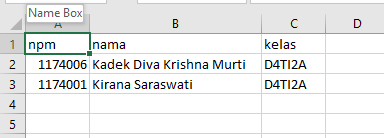
\includegraphics[width=10cm]{figures/4/1174006/Teori/t3.png}
		\centering
	\end{figure}
	
	\item Setelah selesai dibuat, silahkan simpan file tersebut dengan cara mengklik ''File'', lalu klik ''Save''.
	
	\begin{figure}[H]
		\includegraphics[width=10cm]{figures/4/1174006/Teori/t4.png}
		\centering
	\end{figure}
	
	\item Kemudian isi kolom ''File name'' dengan nama file anda dan kolom ''Save as type'' pilih yang berekstensi .csv.
	
	\begin{figure}[H]
		\includegraphics[width=9cm]{figures/4/1174006/Teori/t5.png}
		\centering
	\end{figure}
	
	\item Lalu tinggal klik ''Yes''.
	
	\begin{figure}[H]
		\includegraphics[width=7cm]{figures/4/1174006/Teori/t6.png}
		\centering
	\end{figure}
	
	\item Kemudian file yang Anda telah terbuat tadi tersimpan dengan ekstensi .csv. Untuk melihat isi filenya tinggal klik dua kali pada file tersebut.
	
	\begin{figure}[H]
		
\includegraphics[width=10cm]{figures/4/1174006/Teori/t8.png}
		\centering
	\end{figure}
	
	\item Berikut ini adalah isi dari file yang tadi Anda buat.
	
	\begin{figure}[H]
		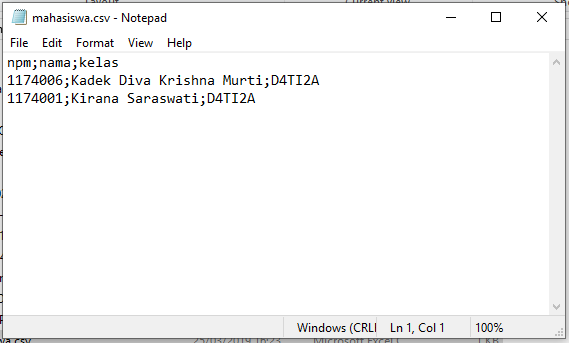
\includegraphics[width=8cm]{figures/4/1174006/Teori/t7.png}
		\centering
	\end{figure}
\end{enumerate}

\textbf{Melihat File CSV di Excel atau Spreadsheet}

\begin{enumerate}
	\item Pertama klik dua kali pada file yang yang berekstensi CSV.
	
	\begin{figure}[H]
		
\includegraphics[width=10cm]{figures/4/1174006/Teori/t8.png}
		\centering
	\end{figure}
	
	\item Kemudian file akan terbuka secara otomatis di aplikasi Excel atau spreadsheet.
	
	\begin{figure}[H]
		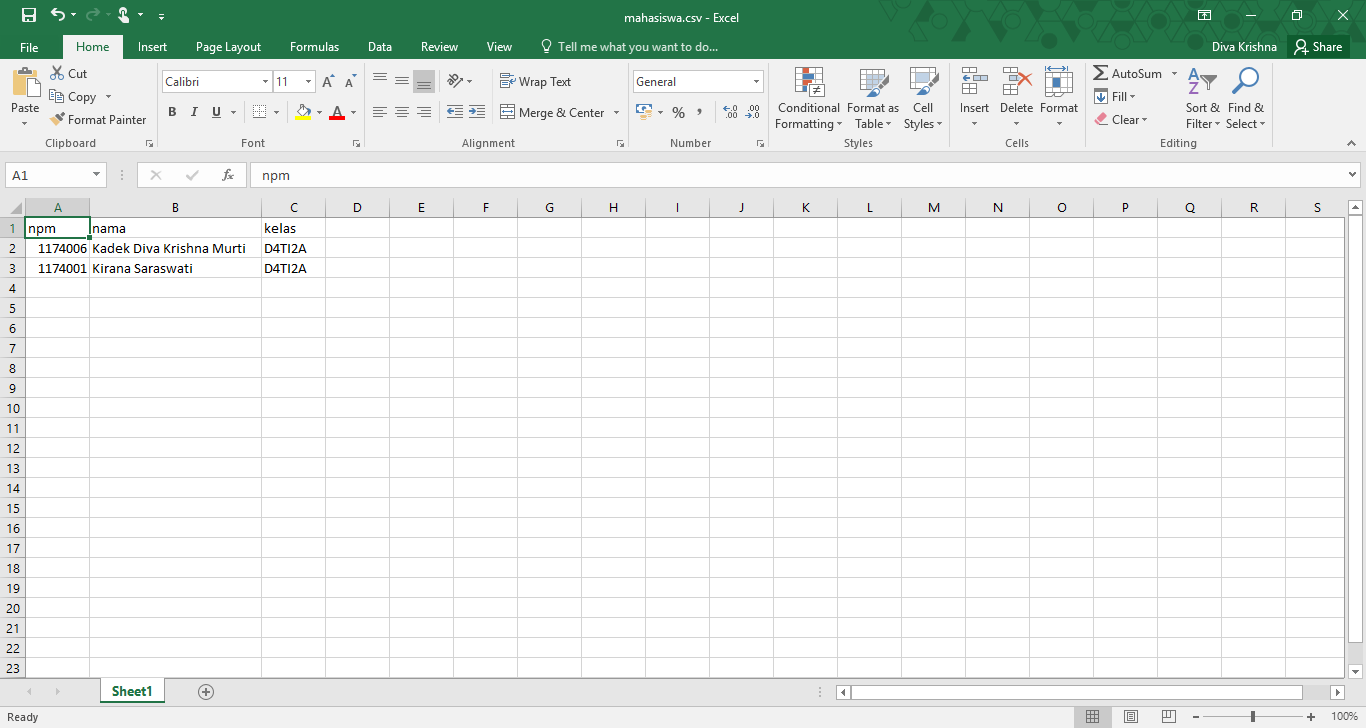
\includegraphics[width=10cm]{figures/4/1174006/Teori/t9.png}
		\centering
	\end{figure}
\end{enumerate}

\subsection{Soal 4}
Sejarah library csv

Library csv mengimplementasikan kelas untuk membaca dan menulis data tabular dalam format CSV. Hal ini memungkinkan programmer untuk mengatakan, "tulis data ini dalam format yang disukai oleh Excel," atau "baca data dari file ini yang dihasilkan oleh Excel," tanpa mengetahui detail yang tepat dari format CSV yang digunakan oleh Excel. Pemrogram juga dapat menggambarkan format CSV yang dipahami oleh aplikasi lain atau menentukan format CSV tujuan khusus mereka sendiri.

\subsection{Soal 5}
Sejarah library pandas

Pada 2008, pengembangan pandas dimulai di AQR Capital Management. Pada akhir 2009 telah menjadi open source, dan secara aktif didukung hari ini oleh komunitas individu yang berpikiran sama di seluruh dunia yang menyumbangkan waktu dan energi berharga mereka untuk membantu membuat panda open source menjadi mungkin.

Sejak 2015, pandas adalah proyek yang disponsori NumFOCUS. Ini akan membantu memastikan keberhasilan pengembangan panda sebagai proyek sumber terbuka kelas dunia.

\subsection{Soal 6}
Fungsi-fungsi yang terdapat di library csv, yaitu:
\begin{enumerate}
	\item reader
	
	Fungsi ini digunakan untuk membaca isi file berformat CSV dari list.
	
	\lstinputlisting[caption = Membaca file berformat CSV list., firstline=7, lastline=13]{src/4/1174006/Teori/1174006.py}
	
	\item DictReader
	
	Fungsi ini digunakan untuk membaca isi file berformat CSV dari dictionary.
	
	\lstinputlisting[caption =  Membaca file berformat CSV dictionary., firstline=15, lastline=21]{src/4/1174006/Teori/1174006.py}
	
	\item write
	
	Fungsi ini digunakan untuk menulis file berformat CSV dari list.
	
	\lstinputlisting[caption =  Menulis file berformat CSV list., firstline=23, lastline=30]{src/4/1174006/Teori/1174006.py}
	
	\item DictWrite
	
	Fungsi ini digunakan untuk menulis file berformat CSV dari dictionary.
	
	\lstinputlisting[caption =  Menulis file berformat CSV dictionary., firstline=32, lastline=41]{src/4/1174006/Teori/1174006.py}
	
\end{enumerate}

\subsection{Soal 7}
Fungsi-fungsi yang terdapat di library pandas, yaitu:
\begin{enumerate}
	\item read\_csv
	
	Fungsi ini digunakan untuk membaca isi file berformat CSV
	
	\lstinputlisting[caption =  Membaca file berformat CSV pandas., firstline=43, lastline=47]{src/4/1174006/Teori/1174006.py}
	
	\item to\_csv
	
	Fungsi ini digunakan untuk menulis file berformat CSV
	
	\lstinputlisting[caption =  Menulis file berformat CSV pandas., firstline=49, lastline=53]{src/4/1174006/Teori/1174006.py}
	
\end{enumerate}

\subsection{Kode Program Teori}
\begin{figure}[H]
	\includegraphics[width=10cm]{figures/4/1174006/Teori/kode_teori1.png}
	\centering
\end{figure}

\begin{figure}[H]
	\includegraphics[width=10cm]{figures/4/1174006/Teori/kode_teori2.png}
	\centering
\end{figure}

\subsection{Cek Plagiat Teori}

\begin{figure}[H]
	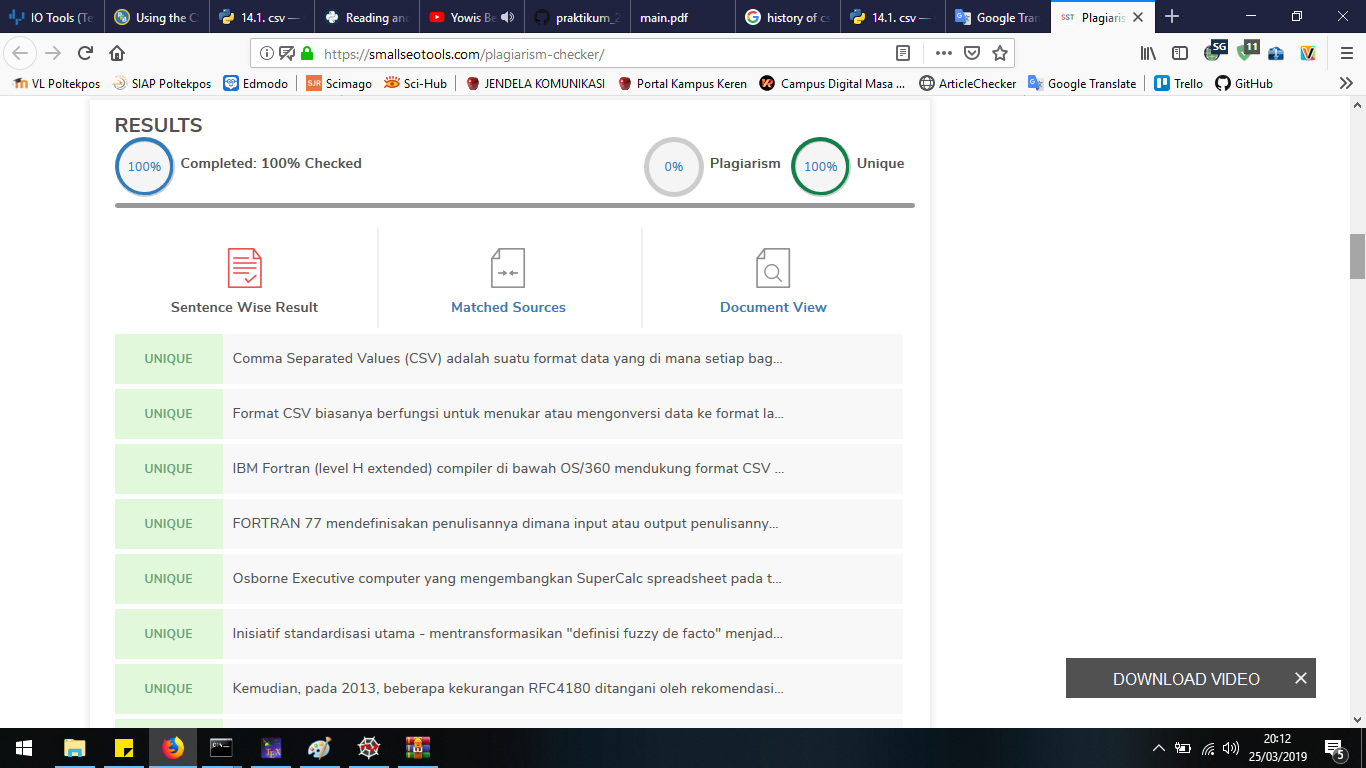
\includegraphics[width=10cm]{figures/4/1174006/Teori/plagiat_teori.png}
	\centering
\end{figure}


\section{Damara Benedikta}
\subsection{Soal 1}
 CSV (Comma Separated Value) merupakan suatu  format basis data sederhana yang dimana setiap record yang ada dipisahkan dengan tanda koma (,) atau titik koma (;). Format data file csv dapat diolah dengan berbagai text editor dengan mudah. Anda tidak perlu (dan Anda tidak akan) membuat pengurai CSV Anda sendiri dari awal. Ada beberapa perpustakaan yang dapat diterima yang dapat Anda gunakan. Pustaka csv Python akan berfungsi untuk sebagian besar kasus. Jika pekerjaan Anda memerlukan banyak data atau analisis numerik, panda library juga memiliki kemampuan penguraian CSV, yang seharusnya menangani sisanya. Dalam bahasa pemrograman Python telah disediakan modul csv yang khusus untuk mengolah data berformat csv.  Untuk memanipulasi data csv dengan python tentunya yang pertama dilakukan adalah mengimport modul csv dengan perintah import csv. File CSV biasanya dibuat oleh program yang menangani sejumlah besar data. Mereka adalah cara yang nyaman untuk mengekspor data dari spreadsheet dan basis data serta mengimpor atau menggunakannya dalam program lain. Misalnya, Anda dapat mengekspor hasil program penambangan data ke file CSV dan kemudian mengimpornya ke dalam spreadsheet untuk menganalisis data, menghasilkan grafik untuk presentasi, atau menyiapkan laporan untuk publikasi. Contoh nya adalah sebagai berikut :

 \lstinputlisting[firstline=8, lastline=20]{src/4/1174012/Teori/damdam.py}

\subsection{Soal 2} 
 Ada beberapa aplikasi yang dapat menciptakan file dengan format csv diantaranya google sheet, number di MacOS dan microsoft excel.

\subsection{Soal 3}
 Cara membuat file csv di excel cukup mudah yaitu :
\begin{itemize}
	\item Buat foldernya
	\item Pilih save as
	\item pilih file dengan format csv
\end{itemize}
Cara membaca file di csv :
\begin{itemize}
	\item Klik data - get external data - form text
	\item Akan muncul Text Import Wizard, arahkan pada file csv yang ingin anda buka lalu Open.
	\item Setelah File terbuka, akan muncul Text Import Wizard.
	\item Pilih Delimited, Kemudian Next (Di sini, bisa juga menentukan baris awal yang akan di import)
	\item Centrang pada Tab dan Comma (Atau sesuai pengaturan File Anda) lalu Next.
	\item Atur Format data pada tiap kolom yang tampil dan klik Finish
\end{itemize}

\subsection{Soal 4}
 CSV digunakan untuk memudahkan data science dan analis karena dinilai terdapat banyak kemudahan yang diperoleh. CSV dapat dimaksimalkan jika dipaduka dengan python karena python adalah bahasa pemrograman yang support ke banyak library termasuk csv. Maka karena itulah perpaduan python dan csv seringkali digunakan oleh perusahaan-perushaan besar dalam mengolah datanya.

\subsection{Soal 5}
Pandas merupakan sebuah tool yang dapat digunakan sebagai alat analisis data dan struktur untuk bahasa pemrograman Python. Pandas dapat mengolah data dengan mudah, salah satu fitur yang ada dalam pandas adalah Dataframe. Fitur dataframe dapat membaca sebuah file dan menjadikannya tabble, juga dapat mengolah suatu data dengan menggunakan operasi seperti join, group by dan teknik lainnya yang terdapat pada SQL. Dalam hal ini pandas tidak jauh beda dengan csv yaitu memiliki keunggulan dalam pengolahan data-data besar dan dapat disupport dengan baik dengan python walaupun mengimport data dalam jumlah banyak.

\subsection{Soal 6}
 Library csv memiliki keunggula-keunggulan dibandingkan format data lainnya merupakah soal kompatibilitas. File csv dapat digunakan, diolah, diekspor/impor, dan dimodifikasi menggunakan berbagai macam perangkat lunak dan bahasa pemrograman. Pada library csv mempunyai fungsi import dan eksport data yang baik dan bisa digunakan dalam jumlah besar.

\subsection{Soal 7}
pandas menyediakan beberapa fungsi operasi untuk mengolah data. Contoh jika menggunakan series bisa mencari nilai max, min, dan mean secara langsung, bahkan juga bisa melakukan operasi perpangkatan pada nilai Series secara langsung.
Pandas dapat mengolah suatu data dan mengolahnya seperti join, distinct, group by, agregasi, dan teknik seperti pada SQL. Hanya saja dilakukan pada tabel yang dimuat dari file ke RAM.


\subsection{bukti bebas plagiarisme}
\begin{figure}[H]
\centering
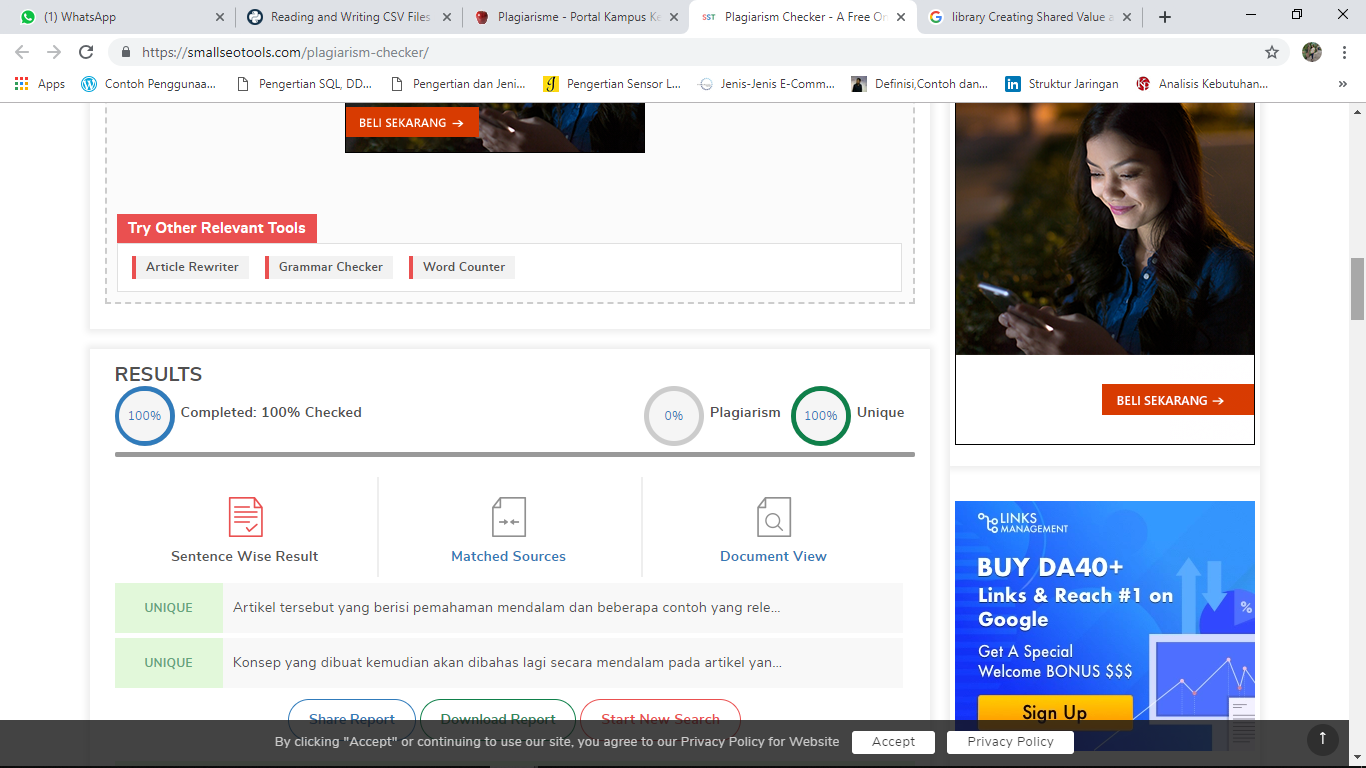
\includegraphics[width=10cm]{figures/4/1174012/Teori/ss1.png}
\caption{SS Bebas Plagiarisme}
\label{damara}
\end{figure}
%%%%%%%%%%%%%%%%%%%%%%%%%%%%%%%%%%%%%%%%%%%%%%
\section{Felix Setiawan Lase}
\subsection{Soal 1}
\textbf{Pengenalan CSV}

File CSV (Nilai Terbatas Koma) adalah jenis file khusus yang dapat Anda buat atau edit di Excel. File CSV menyimpan informasi yang disimpan dengan koma alih-alih menyimpan informasi dalam kolom.

\textbf{Sejarah Format CSV}

Kompiler Fortran IBM (tingkat lanjut H) di bawah OS / 360 mendukung format CSV pada tahun 1972. FORTRAN 77 mendefinisikan penulisannya di mana penulisan input atau output menggunakan koma atau spasi untuk batas antara data dan penulisan disetujui pada tahun 1978.

Pada 2014 IETF menerbitkan RFC7111 yang menjelaskan penerapan fragmen URI dalam dokumen CSV. RFC7111 menentukan bagaimana berbagai baris, kolom, dan sel dapat dipilih dari dokumen CSV menggunakan indeks posisi.

Pada 2015, W3C, dalam upaya meningkatkan CSV dengan semantik formal, menerbitkan rancangan rekomendasi pertama untuk standar metadata CSV, yang dimulai sebagai rekomendasi pada bulan Desember tahun yang sama.

\textbf{Contoh penggunaan format CSV}

\lstinputlisting[caption = Contoh penggunaan format CSV., firstline=1, lastline=3]{src/4/1174026/Teori/teori.csv}

\subsection{Soal 2}
Aplikasi-aplikasi yang dapat menciptkan file csv, yaitu:

\begin{enumerate}
	\item Editor teks (Notepad, Sublime, Atom, dan lain-lain)
	\item Spreadsheet (Microsoft Excel dan lain-lain)
\end{enumerate}

\subsection{Soal 3}
Cara menulis dan membaca file csv di excel atau spreadsheet, sebagai berikut:

\textbf{Menulis File CSV}

\begin{enumerate}
	\item Pertama silahkan buka aplikasi Excel dengan cara klik ''Start'', cari Excel, kemudian tekan Enter.
	
	\begin{figure}[H]
		\includegraphics[width=9cm]{figures/4/1174026/Teori/t1.png}
		\centering
	\end{figure}
	
	\item Setelah aplikasi terbuka silahkan klik ''Blank Workbook''.
	
	\begin{figure}[H]
		\includegraphics[width=10cm]{figures/4/1174026/Teori/t2.png}
		\centering
	\end{figure}
	
	\item Kemudian isi sesuai dengan data yang ingin dibuat.
	
	\begin{figure}[H]
		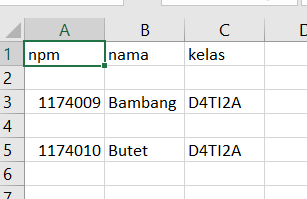
\includegraphics[width=10cm]{figures/4/1174026/Teori/t3.png}
		\centering
	\end{figure}
	
	\item Setelah selesai dibuat, silahkan simpan file tersebut dengan cara mengklik ''File'', lalu klik ''Save''.
	
	\begin{figure}[H]
		\includegraphics[width=10cm]{figures/4/1174026/Teori/t4.png}
		\centering
	\end{figure}
	
	\item Kemudian isi kolom ''File name'' dengan nama file anda dan kolom ''Save as type'' pilih yang berekstensi .csv.
	
	\begin{figure}[H]
		\includegraphics[width=9cm]{figures/4/1174026/Teori/t5.png}
		\centering
	\end{figure}
	
	\item Lalu tinggal klik ''Yes''.
	
	\begin{figure}[H]
		\includegraphics[width=7cm]{figures/4/1174026/Teori/t6.png}
		\centering
	\end{figure}
	
	\item Kemudian file yang Anda telah terbuat tadi tersimpan dengan ekstensi .csv. Untuk melihat isi filenya tinggal klik dua kali pada file tersebut.
	
	\begin{figure}[H]
		
\includegraphics[width=10cm]{figures/4/1174026/Teori/t8.png}
		\centering
	\end{figure}
	
	\item Berikut ini adalah isi dari file yang tadi Anda buat.
	
	\begin{figure}[H]
		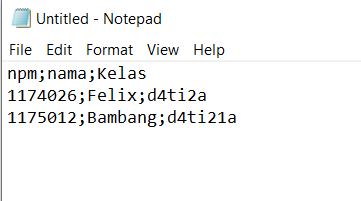
\includegraphics[width=8cm]{figures/4/1174026/Teori/t7.png}
		\centering
	\end{figure}
\end{enumerate}

\textbf{Melihat File CSV di Excel atau Spreadsheet}

\begin{enumerate}
	\item Pertama klik dua kali pada file yang yang berekstensi CSV.
	
	\begin{figure}[H]
		
\includegraphics[width=10cm]{figures/4/1174026/Teori/t8.png}
		\centering
	\end{figure}
	
	\item Kemudian file akan terbuka secara otomatis di aplikasi Excel atau spreadsheet.
	
	\begin{figure}[H]
		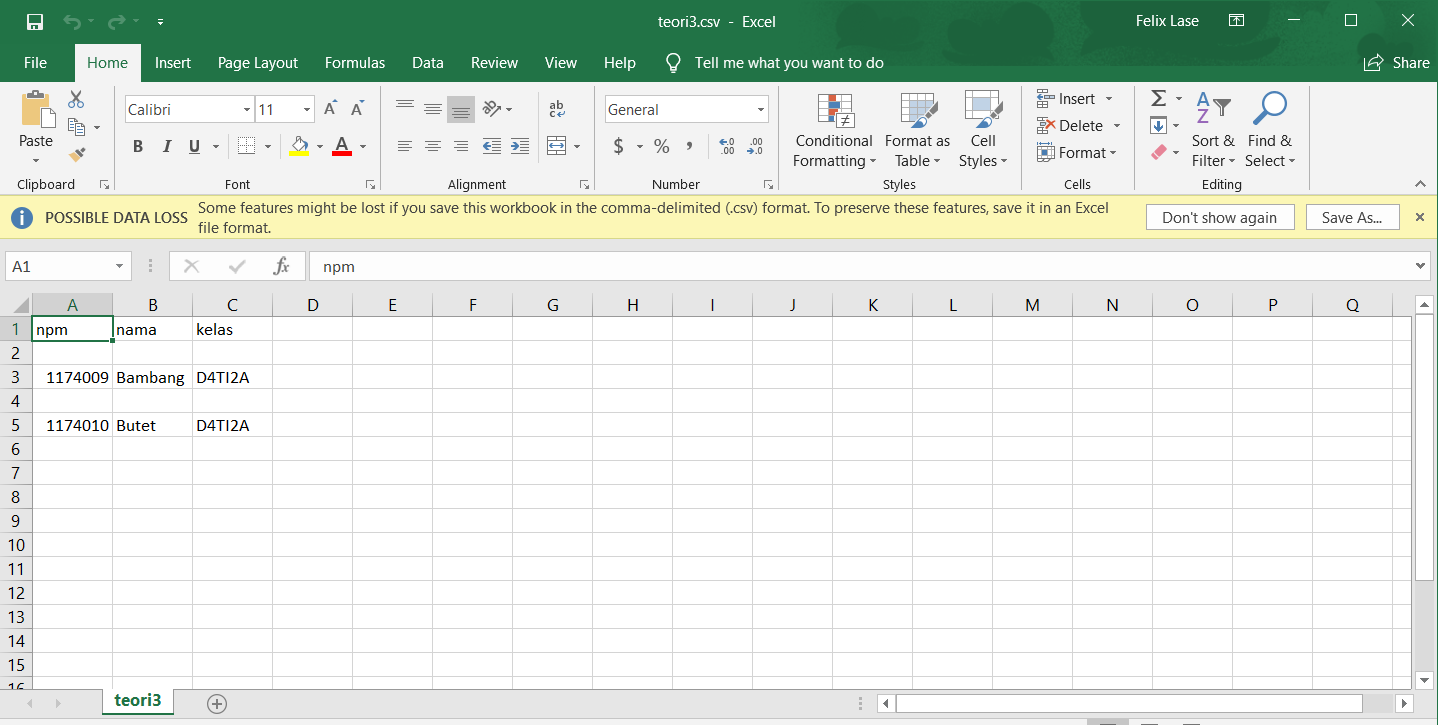
\includegraphics[width=10cm]{figures/4/1174026/Teori/t9.png}
		\centering
	\end{figure}
\end{enumerate}

\subsection{Soal 4}
Sejarah library csv

Perpustakaan CSV mengimplementasikan kelas untuk membaca dan menulis data tabular dalam format CSV. Ini memungkinkan programmer untuk mengatakan, "tulis data ini dalam format yang disukai Excel," atau "baca data dari file ini yang dihasilkan oleh Excel," tanpa mengetahui detail pasti dari format CSV yang digunakan oleh Excel. Pemrogram juga dapat menggambarkan format CSV yang dimengerti oleh aplikasi lain atau menentukan format CSV spesifik mereka sendiri.
	

\subsection{Soal 5}
Sejarah library pandas

Tahun 2008, pengembangan profesional dimulai di AQR Capital Management. Pada akhir 2009 ini telah menjadi open source, dan secara aktif didukung hari ini oleh komunitas individu yang berpikiran sama di seluruh dunia yang menyumbangkan waktu dan energi berharga mereka untuk membantu membuat panda open source menjadi mungkin.

	Sejak tahun 2015, Pandas adalah proyek yang disponsori oleh NumFOCUS. Ini akan membantu memastikan keberhasilan pengembangan Panda sebagai proyek open source kelas dunia.
	

\subsection{Soal 6}
Fungsi-fungsi yang terdapat di library csv, yaitu:
\begin{enumerate}
	\item reader
	
	Fungsi ini digunakan untuk membaca isi file berformat CSV dari list.
	
	\lstinputlisting[caption = Membaca file berformat CSV list., firstline=7, lastline=13]{src/4/1174026/Teori/1174026.py}
	
	\item DictReader
	
	Fungsi ini digunakan untuk membaca isi file berformat CSV dari dictionary.
	
	\lstinputlisting[caption =  Membaca file berformat CSV dictionary., firstline=15, lastline=21]{src/4/1174026/Teori/1174026.py}
	
	\item write
	
	Fungsi ini digunakan untuk menulis file berformat CSV dari list.
	
	\lstinputlisting[caption =  Menulis file berformat CSV list., firstline=23, lastline=30]{src/4/1174026/Teori/1174026.py}
	
	\item DictWrite
	
	Fungsi ini digunakan untuk menulis file berformat CSV dari dictionary.
	
	\lstinputlisting[caption =  Menulis file berformat CSV dictionary., firstline=32, lastline=41]{src/4/1174026/Teori/1174026.py}
	
\end{enumerate}

\subsection{Soal 7}
Fungsi-fungsi yang terdapat di library pandas, yaitu:
\begin{enumerate}
	\item read\_csv
	
	Fungsi ini digunakan untuk membaca isi file berformat CSV
	
	\lstinputlisting[caption =  Membaca file berformat CSV pandas., firstline=43, lastline=47]{src/4/1174026/Teori/1174026.py}
	
	\item to\_csv
	
	Fungsi ini digunakan untuk menulis file berformat CSV
	
	\lstinputlisting[caption =  Menulis file berformat CSV pandas., firstline=49, lastline=53]{src/4/1174026/Teori/1174026.py}
	
\end{enumerate}

\subsection{Kode Program Teori}
\begin{figure}[H]
	\includegraphics[width=10cm]{figures/4/1174026/Teori/kode_teori1.png}
	\centering
\end{figure}

\begin{figure}[H]
	\includegraphics[width=10cm]{figures/4/1174026/Teori/kode_teori2.png}
	\centering
\end{figure}

\subsection{Cek Plagiat Teori}

\begin{figure}[H]
	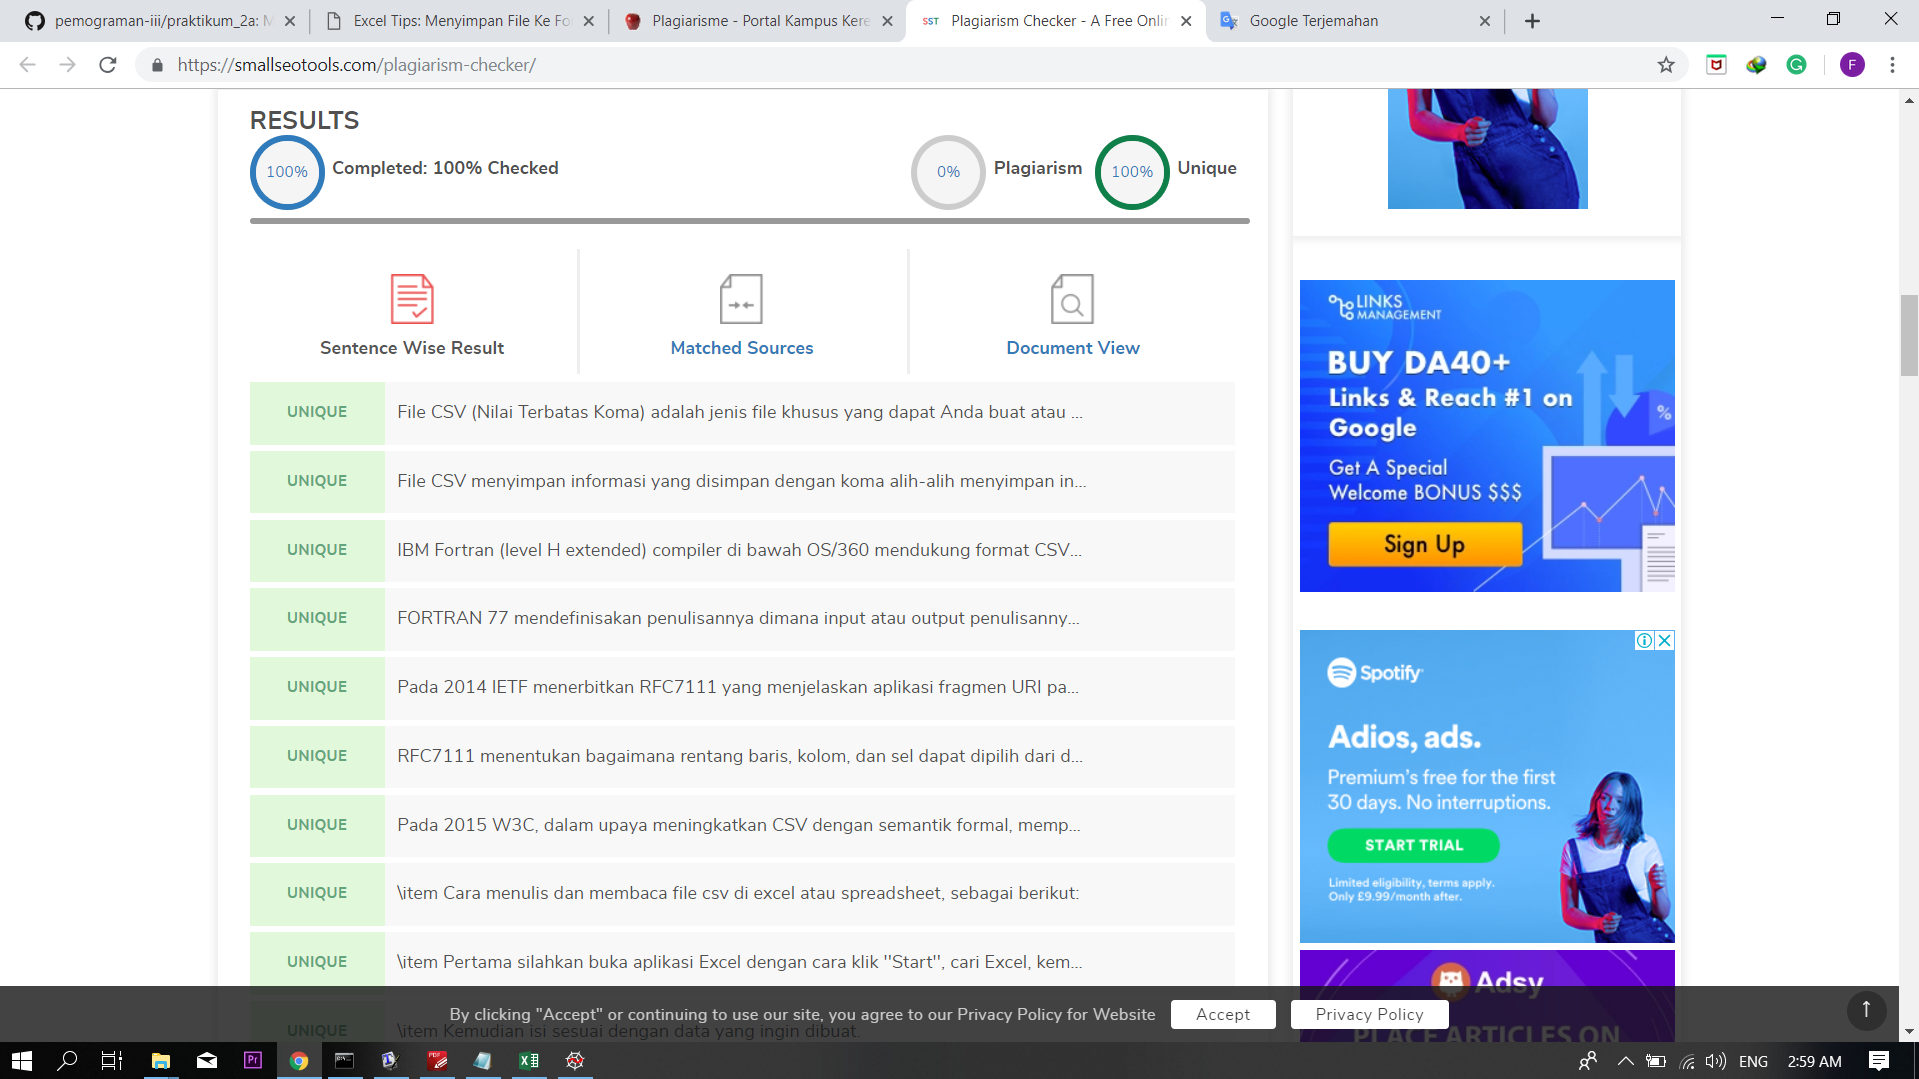
\includegraphics[width=10cm]{figures/4/1174026/Teori/plagiat_teori.png}
	\centering
\end{figure}
%%%%%%%%%%%%%%%%%%%%%%%%%%%%%%%%%%%%%%%%%%%%%

\section{Harun Ar-Rasyid}
\subsection{Soal 1}
Isi jawaban soal ke-1

Kalau mau dibikin paragrap \textbf{cukup enter aja}, tidak usah pakai \verb|par| dsb

%\subsection{Soal 2}
%Isi jawaban soal ke-2

%\subsection{Soal 3}
%Isi jawaban soal ke-3

\section{Sri Rahayu}
\subsection{Soal 1}
Isi jawaban soal ke-1

Kalau mau dibikin paragrap \textbf{cukup enter aja}, tidak usah pakai \verb|par| dsb

%\subsection{Soal 2}
%Isi jawaban soal ke-2

%\subsection{Soal 3}
%Isi jawaban soal ke-3

\section{Doli Jonviter}
\subsection{Soal 1}
Isi jawaban soal ke-1

Kalau mau dibikin paragrap \textbf{cukup enter aja}, tidak usah pakai \verb|par| dsb

%\subsection{Soal 2}
%Isi jawaban soal ke-2

%\subsection{Soal 3}
%Isi jawaban soal ke-3

\section{Rahmatul Ridha}
\subsection{Soal 1}
Isi jawaban soal ke-1

Kalau mau dibikin paragrap \textbf{cukup enter aja}, tidak usah pakai \verb|par| dsb

%\subsection{Soal 2}
%Isi jawaban soal ke-2

%\subsection{Soal 3}
%Isi jawaban soal ke-3

\section{Tomy Prawoto}
\subsection{Soal 1}
Isi jawaban soal ke-1

Kalau mau dibikin paragrap \textbf{cukup enter aja}, tidak usah pakai \verb|par| dsb

%\subsection{Soal 2}
%Isi jawaban soal ke-2

%\subsection{Soal 3}
%Isi jawaban soal ke-3
